\pagebreak
\section{Scope and Content of this Document}

\par This document has been developed to provide guidance to ECCO V4r4 data users for easily navigating the list of available datasets. It offers an overview of the ECCO V4r4 datasets, including the data storage format, filename conventions, supporting metadata conventions, and the structure of data product files.

\par Descriptions are provided for NetCDF data files, including global attributes, dimensions, coordinates, and variable metadata. Additionally, detailed descriptions are included for each ECCO V4r4 dataset: the native Lat-Lon-Cap 90 (LLC90) grid, the regular 0.5-degree latitude-longitude grid, and the one-dimensional dataset. Grid geometry details are also provided for both the native LLC90 grid and the 0.5-degree latitude-longitude grid configurations. Illustrative figures accompany each section to enhance understanding.


% \par\vspace{0.25cm}
% \begin{figure}[h]
%     \centering
%     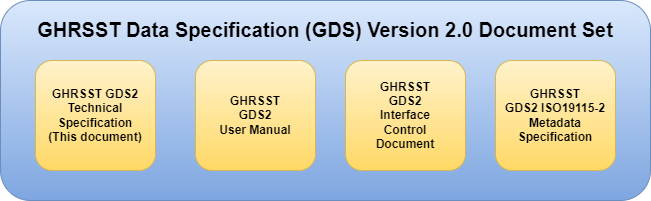
\includegraphics[width=1 \textwidth]{../images/schematicOverview.drawio.png}
%     \caption{Schematic overview of the GHRSST Data Specification Version 2.0 document pack.}
%     \label{fig:schematic_overview}
% \end{figure}